\section{User Interface Design}

\subsection{UX Diagram}

\begin{figure}[H]
	\centering
	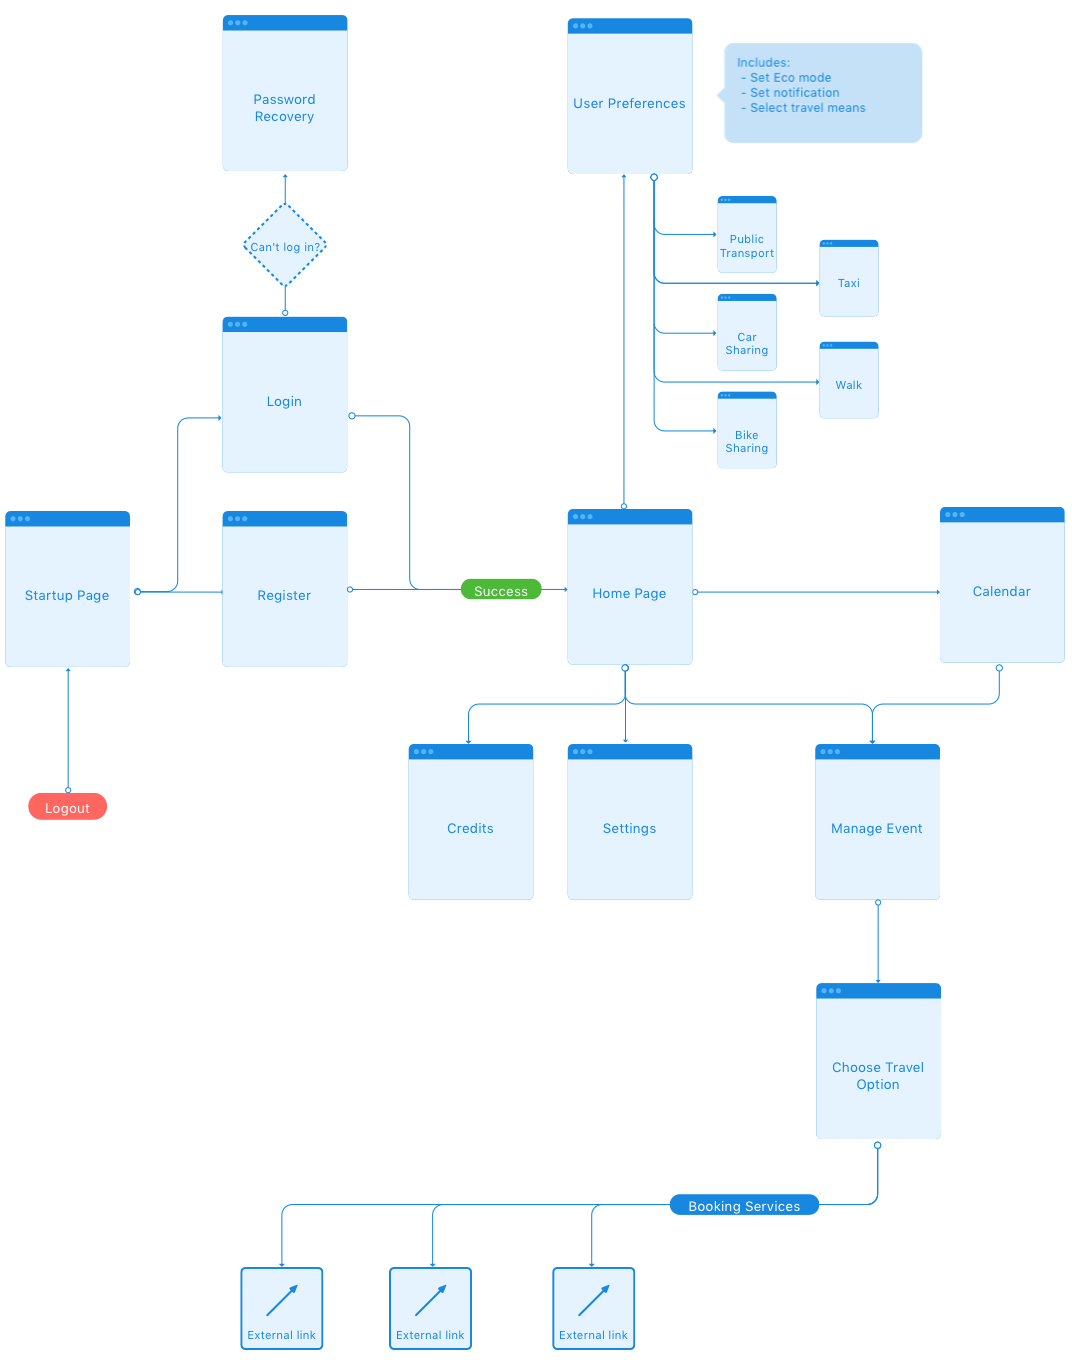
\includegraphics[scale=0.70]{uxdiagram.png}
	\caption{UX diagram}
\end{figure}

For the User Interface Design, we refer to section 3.1.1 of the RASD document. In this section, we enrich what was shown in the RASD by means of a User Experience diagram, which is principally thought to explain as clearly as possible the relationships between the various sections of the application.\\ \\
As we can see from the diagram, the leftmost part is merely devoted to the necessary operations to log into the application:

\begin{itemize}
	\item \textit{Startup Page}
	\item \textit{Login}
	\item \textit{Register}
	\item \textit{Password Recovery}
\end{itemize}

The main window of the application is the \textit{Home Page}, which occupies a central position in the diagram. In this window user related information and daily schedule are displayed, any other section is reachable trough a sidebar.
The sections arranged around the \textit{Home Page} are:

\begin{itemize}
	\item \textit{User Preferences:} users are able to customize their travel experience.
	\item \textit{Credits:} references to the creators of the application.
	\item \textit{Settings:} mail, password and username can be edited.
	\item \textit{Calendar:} displays a view of the user calendar per month. If a day has at least one event scheduled, a bullet is shown on the day cell.
\end{itemize}

As already outlined in the RASD, from the \textit{Home Page} or the \textit{Calendar} section is possible add, edit or delete an event in the dedicated \textit{Manage Event} section. Once specified all the relevant information, the application will lead to the \textit{Choose Travel Option} section, where a list of available travel means is provided together with links to external booking services to purchase tickets and rides.